\documentclass[12pt,a4paper]{article}
\usepackage[UTF8]{ctex}
\usepackage{amsmath,amssymb}
\usepackage{listings}
\usepackage{xcolor}
\usepackage{hyperref}
\usepackage{geometry}
\usepackage{graphicx}
\geometry{margin=2.5cm}

\lstdefinestyle{python}{
  language=Python,
  basicstyle=\ttfamily\small,
  keywordstyle=\color{blue}\bfseries,
  commentstyle=\color{gray},
  stringstyle=\color{red},
  showstringspaces=false,
  breaklines=true,
  frame=single,
  backgroundcolor=\color{gray!10}
}

\title{Grover Search / Grover 搜索}
\author{QuoNic}
\date{}

\begin{document}
\maketitle

\begin{center}
\textbf{Algorithms / 算法} | 难度：中级 | 预计时间：10 分钟
\end{center}

\tableofcontents
\newpage

%% ============================================================
\section{为什么需要？}

在无序数据库中查找目标，经典算法需要 $O(N)$ 次查询，Grover 算法只需要 $O(\sqrt{N})$ 次。

\subsection{经典局限}
\begin{itemize}
  \item 经典搜索：最坏情况需要遍历所有 $N$ 个元素
  \item 对于 $N=10^6$，经典需要 $10^6$ 次，量子只需要 $10^3$ 次
\end{itemize}

\subsection{量子优势}
\begin{itemize}
  \item 二次加速：$O(\sqrt{N})$ vs $O(N)$
  \item 对于大规模搜索问题，加速效果显著
  \item 是许多量子算法的基础（振幅放大、量子计数）
\end{itemize}

\subsection{实际应用}
\begin{itemize}
  \item 数据库搜索
  \item 密码学（搜索密钥空间）
  \item 优化问题（寻找最优解）
  \item SAT 求解
\end{itemize}

%% ============================================================
\section{快速上手}

\begin{lstlisting}[style=python]
from quonic.algorithms import grover

# Search for |11> in 2-qubit space
result = grover("11", 2, shots=1024)
print(result.counts)
\end{lstlisting}

\textbf{预期输出}：
\begin{verbatim}
{'11': 1008, '00': 6, '01': 5, '10': 5}
\end{verbatim}

%% ============================================================
\section{原理详解}

\subsection{电路图}

\begin{center}
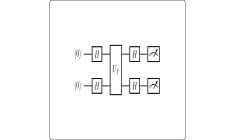
\includegraphics[width=0.6\textwidth]{../../images/grover_circuit.svg}
\end{center}

\subsection{数学推导}

\textbf{Step 1: 初始化}

对所有量子比特施加 $H$ 门，创建均匀叠加态：
\begin{equation}
|\psi_0\rangle = \frac{|00\rangle + |01\rangle + |10\rangle + |11\rangle}{2}
\end{equation}

\textbf{Step 2: Oracle 标记}

Oracle 翻转目标态 $|11\rangle$ 的相位：
\begin{equation}
|\psi_1\rangle = \frac{|00\rangle + |01\rangle + |10\rangle - |11\rangle}{2}
\end{equation}

\textbf{Step 3: Diffusion 算子}

Diffusion 算子关于平均振幅反射：
\begin{equation}
\text{avg} = \frac{1/4 + 1/4 + 1/4 - 1/4}{4} = \frac{1}{8}
\end{equation}

反射后：$|11\rangle$ 的振幅被放大。

\textbf{Step 4: 迭代}

重复 Oracle + Diffusion，每次迭代都放大目标态的振幅。

最优迭代次数 $\approx \pi\sqrt{N}/4$，测量后目标态概率 $\approx 100\%$。

\subsection{几何解释}

Grover 算法的几何解释：
\begin{enumerate}
  \item 初始态在均匀叠加态空间中
  \item Oracle 标记目标态，翻转其相位
  \item Diffusion 关于平均振幅反射
  \item 每次迭代，目标态的振幅被放大
  \item 经过 $\sim\sqrt{N}$ 次迭代，目标态概率接近 100\%
\end{enumerate}

%% ============================================================
\section{代码详解}

\begin{lstlisting}[style=python]
from quonic.algorithms import grover

# grover(target, n_qubits, shots)
# target: target bit string
# n_qubits: number of qubits
# shots: number of measurements
result = grover("11", 2, shots=1024)

# result.counts: measurement statistics
print(result.counts)
\end{lstlisting}

%% ============================================================
\section{进阶用法}

\subsection{场景 1：多量子比特搜索}

\begin{lstlisting}[style=python]
# Search for |101> in 3-qubit space
result = grover("101", 3, shots=1024)
print(result.counts)
\end{lstlisting}

\subsection{场景 2：多目标搜索}

\begin{lstlisting}[style=python]
# Search for multiple targets
from quonic.algorithms import grover_multi
result = grover_multi(["00", "11"], 2, shots=1024)
print(result.counts)
\end{lstlisting}

\subsection{场景 3：Grover 搜索用于优化}

\begin{lstlisting}[style=python]
# Grover for optimization
# Find optimal solution in 4 options
result = grover("11", 2, shots=1024)
# |11> corresponds to optimal solution
\end{lstlisting}

%% ============================================================
\section{适用场景}

\subsection{数据库搜索}

在无序数据库中查找目标，经典需要 $O(N)$，量子只需要 $O(\sqrt{N})$。

\subsection{密码学}

搜索密钥空间，可以加速暴力破解。

\subsection{优化问题}

寻找最优解，可以加速组合优化问题的求解。

%% ============================================================
\section{常见问题}

\subsection{Grover 搜索的加速比是多少？}

二次加速：$O(\sqrt{N})$ vs $O(N)$。对于 $N=10^6$，经典需要 $10^6$ 次，量子只需要 $10^3$ 次。

\subsection{Grover 搜索需要多少次迭代？}

最优迭代次数 $\approx \pi\sqrt{N}/4$。对于 $N=4$（2 量子比特），只需要 1 次迭代。

\subsection{Grover 搜索能找到所有目标吗？}

Grover 搜索只能找到一个目标。如果需要找所有目标，需要多次运行。

%% ============================================================
\section{学习路径}

\subsection{前置知识}
\begin{itemize}
  \item 量子比特和叠加态
  \item Hadamard 门和 CNOT 门
  \item 量子测量
\end{itemize}

\subsection{继续学习}
\begin{itemize}
  \item 振幅放大（Grover 的推广）
  \item 量子计数（计算目标数量）
  \item 量子优化算法
\end{itemize}

%% ============================================================
\section{完整示例代码}

\subsection{示例 1：基本 Grover 搜索}

\begin{lstlisting}[style=python]
from quonic.algorithms import grover

result = grover("11", 2, shots=1024)
print(result.counts)
\end{lstlisting}

\subsection{示例 2：3 量子比特 Grover 搜索}

\begin{lstlisting}[style=python]
from quonic.algorithms import grover

result = grover("101", 3, shots=1024)
print(result.counts)
\end{lstlisting}

\end{document}
